\documentclass[20pt]{article}

\usepackage{fancyhdr}
\usepackage[a4paper, margin=2cm]{geometry}
\usepackage{titlesec}
\usepackage{amsmath}
\usepackage{amssymb}
\usepackage{enumitem}
\usepackage{times}
\usepackage{tipa}
\usepackage{phonrule}
\usepackage{covington}
\usepackage{color}
\usepackage{bussproofs}
\usepackage{tikz-qtree}
\usepackage{stmaryrd}

\setlength\parindent{0pt}
\titlespacing*{\section}{0pt}{0.7\baselineskip}{0.7\baselineskip}
\titleformat*{\section}{\large\bfseries}

\newcommand{\ipa}[1]{\textipa{#1}}
\newcommand{\broad}[1]{/\ipa{#1}/}
\newcommand{\narrow}[1]{[ \ipa{#1} ]}
\newcommand{\english}[1]{$<$#1$>$}
\newcommand{\sk}[0]{{\kern 0.05em}}
\newcommand{\mk}[0]{{\kern 0.1em}}
\newcommand{\smallcapi}[0]{\sk\textsci\sk}
\newcommand{\openo}[0]{\sk O}
\newcommand{\marked}[1]{\textsc{#1}}
\newcommand{\trans}[3]{\lq #1\rq \mk \narrow{#2} $\rightsquigarrow$ \narrow{#3}}
\newcommand{\brackets}[1]{\ensuremath{\llbracket \text{#1}\rrbracket^{c}}}
\newcommand{\card}[1]{\ensuremath{| #1 |}}

\pagestyle{fancy}
\lhead{Alice McKean}
\rhead{\thepage}
\cfoot{}

\begin{document}

\begin{titlepage}
    \begin{center}
        \vspace*{1cm}
 
        \Huge
        \textbf{Introduction to Lingusitic Analysis Final}
 
        \vspace{0.5cm}
        \LARGE
        Part One
 
        \vspace{0.5cm}
 
        \textbf{Alice McKean}
 
        \vfill
 
        \Large
        Reed College\\
        \today
    \end{center}
\end{titlepage}

\section{Morphological Analysis}

\begin{tabular}{rl|rl|rl|ll|ll|ll}
    \multicolumn{2}{c|}{-3 Subject} & \multicolumn{2}{c|}{-2 Polarity}
  & \multicolumn{2}{c|}{-1 Object}  & \multicolumn{2}{c|}{+0 Root}
  & \multicolumn{2}{c|}{+1 Object}  & \multicolumn{2}{c }{+2 Tense} \\
  \hline
    \ipa{\o}-   & `3'      & \ipa{\o}- & `POS'      & \ipa{\o}-   &
  & \ipa{ba}    & `to go'  & -\ipa{\o} &            & -\ipa{ke}   & `PAST' \\

    \ipa{Na}-   & `1SG'    & \ipa{ma}- & `NEG'      & \{\ipa{ra}- \ipa{ja}- \ipa{jara}-\} & `3PL'
  & \ipa{r\~Wh} & `to see' & -\ipa{na} & `1SG'      & -\ipa{keo}  & `PAST 3SG SUB' \\
  
    \ipa{n@}-   & `2SG'    &           &            &             &
  &             &          & -\ipa{ni} & `2SG'      & -\ipa{ker@} & `PAST 3PL SUB' \\

    \ipa{ge}-   & `1PL'    & & & & & & & -\ipa{si}  & `1PL'       & -\ipa{ja}  & `FUT' \\

    \ipa{dze}-  & `2PL'    & & & & & & & -\ipa{tsi} & `2PL'       & -\ipa{wa}  & `FUT 3SG SUB' \\
  
                &          & & & & & & &            &             & -\ipa{rja} & `FUT 3PL SUB' \\
\end{tabular} 

\vspace{1em}

The main instance of allomorphy in this data set is the morphemes for third
person plural objects. These are \{\ipa{ra}- \ipa{ja}- \ipa{jara}-\} with the first two
seemingly interchangeable. The last morpheme only appears in the data set when the
subject and object are both third person plural. In that case the information
that the subject is third person plural is reflected in the tense morpheme. This
could mean that it carries more information than the others but more data would
need to be provided to make a distinction. \\

This language nominative-accusative as the subject person morphemes are the same
when used in a transitive verb or used in an intransitive verb. While the object
person morphemes are different from the subject morphemes (\ipa{Na} vs
\ipa{na}).

\section{Phrase Structure Trees}

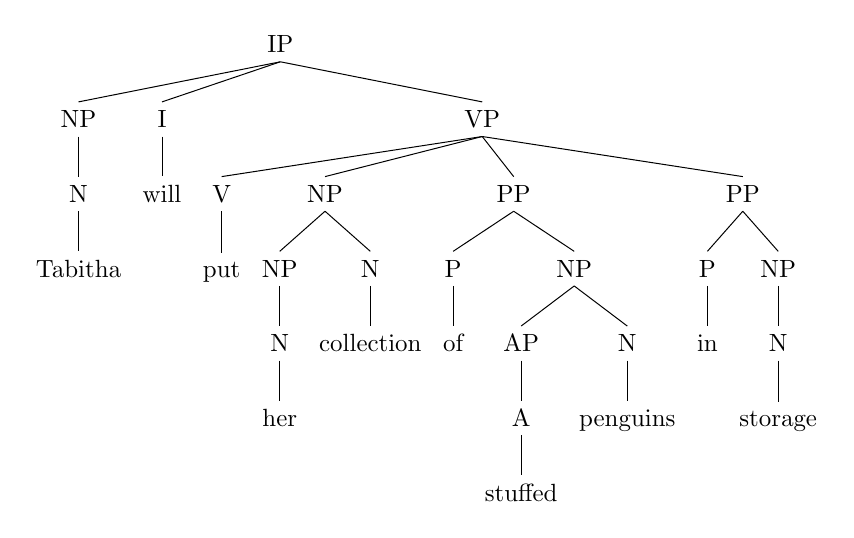
\begin{tikzpicture}[scale=0.9, transform shape]
  \Tree [.IP [.NP [.N Tabitha ] ]
             [.I  will ]
             [.VP [.V put ]
                  [.NP [.NP [.N her ] ]
                       [.N collection ]
                  ]
                  [.PP [.P of ]
                       [.NP [.AP [.A stuffed ] ]
                            [.N penguins ]
                       ]
                  ]
                  [.PP [.P in ]
                       [.NP [.N storage ] ]
                  ]
             ]
        ]
\end{tikzpicture}

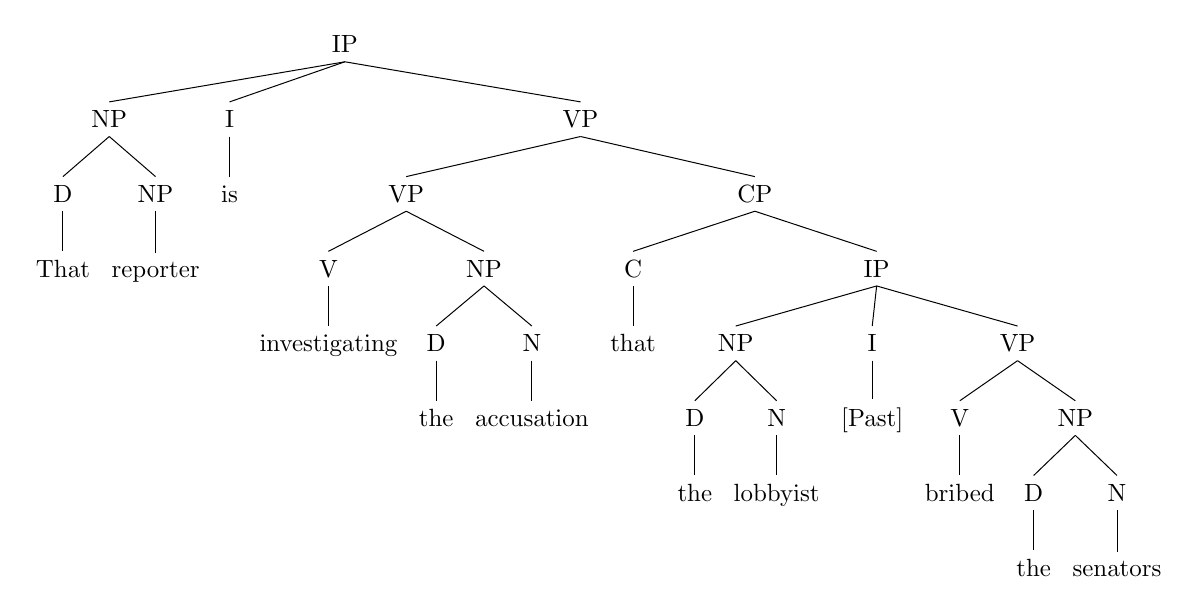
\begin{tikzpicture}[scale=0.9, transform shape]
  \Tree [.IP [.NP [.D That ]
                  [.NP reporter ]
             ]
             [.I  is ]
             [.VP [.VP [.V investigating ]
                       [.NP [.D the ]
                            [.N accusation ]
                       ]
                  ]
                  [.CP [.C that ]
                       [.IP [.NP [.D the ]
                                 [.N lobbyist ]
                            ]
                            [.I  [.[Past] ] ]
                            [.VP [.V bribed ]
                                 [.NP [.D the ]
                                      [.N senators ]
                                 ]
                            ]
                       ]
                  ]
             ]
        ]
\end{tikzpicture}

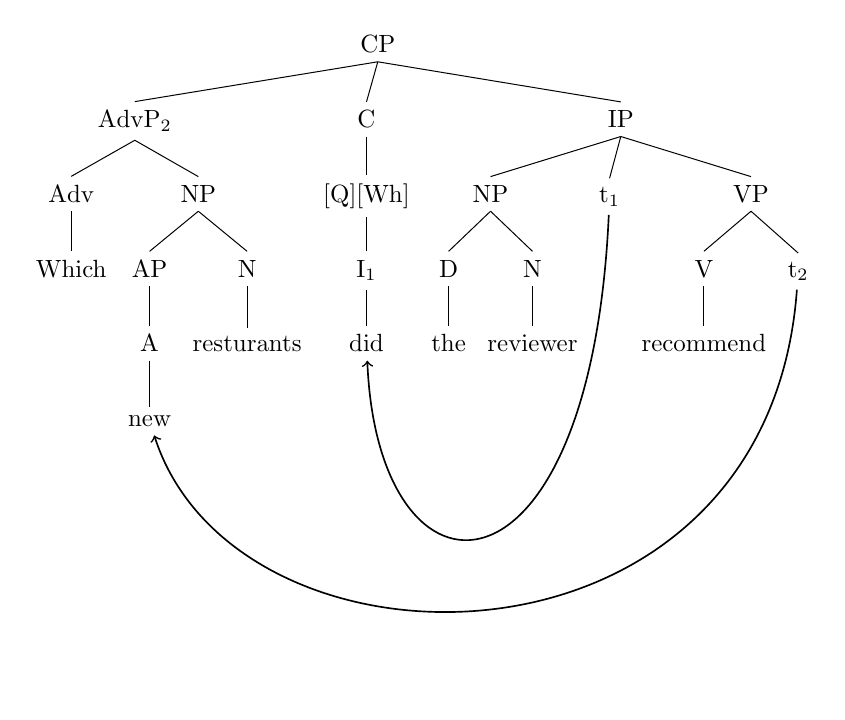
\begin{tikzpicture}[scale=0.9, transform shape]
  \Tree [.CP [.AdvP$_2$ [.Adv Which ]
                        [.NP [.AP [.A \node(wh){new}; ]]
                             [.N resturants ]
                        ]
             ]
             [.C  [.[Q][Wh] [.I$_1$ \node(aux){did}; ] ] ]
             [.IP [.NP [.D the ]
                       [.N reviewer ]
                  ]
                  [.\node(t1){t$_1$}; ]
                  [.VP [.V recommend ]
                       [.\node(t2){t$_2$}; ]
                  ]
             ]
        ]
\draw[semithick,->] (t1)..controls (3,-8) and (0,-8)..(aux);
\draw[semithick,->] (t2)..controls (5.5,-9) and (-2,-9)..(wh);
\end{tikzpicture}

\begin{tikzpicture}[scale=0.9, transform shape]
  \Tree [.CP [.AdvP$_2$ [.Adv \node(wh){What}; ]
             ]
             [.C  [.[Q][Wh] [.I$_1$ \node(aux){do}; ] ] ]
             [.IP [.NP [.N you ] ]
                  [.\node(t1){t$_1$}; ]
                  [.VP [.V suppose ]
                       [.CP [.C that ]
                            [.IP [.NP [.N Norbert ] ]
                                 [.I  [.[Pres] ] ]
                                 [.VP [.VP [.V wants ]
                                           [.\node(t2){t$_2$}; ]
                                      ]
                                      [.PP [.P for ]
                                           [.NP [.NP [.N his ] ]
                                                [.N birthday ]
                                           ]
                                      ]
                                 ]
                            ]
                       ]
                  ]
             ]
        ]

\draw[semithick,->] (t1)..controls (1.5,-6) and (0,-6)..(aux);
\draw[semithick,->] (t2)..controls (8,-12) and (-2.5,-12)..(wh);
\end{tikzpicture}

\newpage

\section{Syntactic Argumentation}

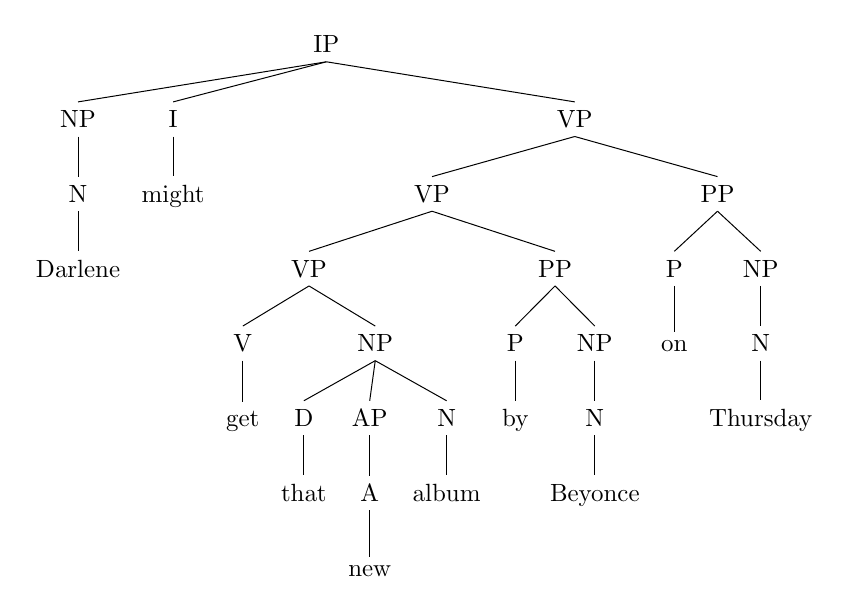
\begin{tikzpicture}[scale=0.9, transform shape]
  \Tree [.IP [.NP [.N Darlene ] ]
             [.I  might ]
             [.VP [.VP [.VP [.V get ]
                            [.NP [.D that ]
                                 [.AP [.A new ] ]
                                 [.N album ]
                            ]
                       ]
                       [.PP [.P by ]
                            [.NP [.N Beyonce ] ]
                       ]
                  ]
                  [.PP [.P on ]
                       [.NP [.N Thursday ] ]
                  ]
             ]
        ]
\end{tikzpicture}

This constituent structure only differs in the mother of the last preposition
phrase. This structure allows for a do so replacement of the last half of the
sentence. ``Darlene might do so'' is a grammatical sentence under Tree B but is not allowed
under Tree A. In a similar vain as before the last half of the sentence can be
pseudo clefted. ``What Darlene might do is get that new album by Beyonce on
Thursday'' and ``Get that new album by Beyonce on Thursday is what Darlene
might do'' are both grammatical sentences under Tree B but not possible under
Tree A. A response to the question ``What might Darlene do'' is ``get that new
album by Beyonce on Thursday''. If the last preposition is not in the verb
phrase you can't inclued the ``on Thursday'' part.

\section{Semantics}

\begin{enumerate}[label=(\alph*)]
  \item
    \begin{enumerate}[label=(\arabic*)]
      \setcounter{enumii}{4}
      \item B entails and presupposes A because B meets the condition ($\ge1$
        Hungarian semanticist) for A to be true.
      \item A entails and presupposes B because B can be thought of as a pseudo
        projection of the two truth values in A.
      \item A does not entail B because there are contexts in which its true
        that not every student got the right answer while also no student got
        the right answer. Similarly B does not entail A because there are
        contexts in which its true some students got the right answer while the
        whole class got the right answer. It could be argued that the two
        sentences implicate each other. Imagine a professor trying to explain
        how hard a test will be. Therefore this question would fall into none of
        the above.
      \item B entails and presupposes A as A is just a rewording of the first
        clause of sentence B.
    \end{enumerate}
  \item
    \begin{enumerate}[label=(\alph*)]
      \item $\card{\brackets{NP} \cap \brackets{VP}} \ge m \cdot
        \card{\brackets{NP}}$ \\
        Where m is a percentage of ``mostness''. It would be very hard to find a
        universal percentage for ``mostness''. This definition and any other
        definition wouldn't be able to precisely pin down what humans mean by most.
      \item $\card{\brackets{NP} \cap \brackets{VP}} \le 12$
      \item $\brackets{NP} \subseteq \brackets{VP} \wedge \card{\brackets{NP}} = 2$
      \item $\card{\brackets{NP} \cap \brackets{VP}} > m$ \\
        Where m is a number representing counting how many items humans consider
        ``many'' to be. This definiton suffers from the same problem as the
        first definiton.
    \end{enumerate}
  \item
    $\text{NP}' = \brackets{Somali students} \subseteq \brackets{students}$ \\
    ``Exactly two Somali students are vegan'' does not entail ``Exactly two
    students are vegan'' because there could be non Somali students who are
    vegans. Similarly ``Exactly two students are vegan'' does not entail
    ``Exactly two Somali students are vegan'' because the first two students
    could not be Somali. This means that the quantifier ``Exactly two'' is not
    increasing or decreasing with respect to the NP.

    $\text{VP}' = \brackets{religous vegans} \subseteq \brackets{vegans}$ \\
    For a similar reason as above the quantifier ``Exactly two'' is not
    increasing or decreasing with respect to the VP.
\end{enumerate}

\newpage

\newpage
\begin{center}
  \thispagestyle{empty}
  This page was intentionally left blank.
\end{center}
\newpage


\begin{titlepage}
    \begin{center}
        \vspace*{1cm}
 
        \Huge
        \textbf{Introduction to Lingusitic Analysis Final}
 
        \vspace{0.5cm}
        \LARGE
        Part Two
 
        \vspace{0.5cm}
 
        \textbf{Alice McKean}
 
        \vfill
 
        \Large
        Reed College\\
        \today
    \end{center}
\end{titlepage}

\section{Phonetics}

\textbf{Broad Transcription}
\vspace{0.7em}

\broad{
  s\sk @m"tAI\sk mz wi k\ae n fAI\sk nd It "izi tu f\textrhookschwa "g3t @"baUt
  Di "sAl@d g\*raUnd bI"n@T "aU\textrhookschwa \mk \mk fit b2t wi m2st
  ri"m@mb\textrhookschwa D\ae t "wi\textrhookschwa \mk \mk I\sk n D@ steIt w\textrhookschwa
  \mk \mk D@ r3d kleI g\sk Ivz laIf tU \textdyoghlig 3"n\textrhookschwa aIS@nz
  2v "drim\textrhookschwa z d@ steIt w\textrhookschwa \mk \mk "mArtI\sk n
  mAr\textteshlig d An "bAlIt bAksz \ae nd \textteshlig \ae l@n\textdyoghlig d A
  "neIS@nz "kAnS@ns A "\textdyoghlig O\*r\textdyoghlig @ D\ae t geIv 2s D@
  "gAdfAD\textrhookschwa \mk \mk 2v sOl D@ kwin 2v D@ m3t \ae nd s3nt A "pin2t
  "fA\*rm\textrhookschwa \mk \mk \mk tu D@ "Ov@l "Of@s D\ae t Iz "aU\textrhookschwa
  \mk \mk "\textdyoghlig O\*r\textdyoghlig @
} \\

\textbf{Narrow Transcription}
\begin{enumerate}
  \item \narrow{"k\super hwzaIk\ae T@R\textrhookschwa \sk \textltilde aIk}
  \item \narrow{n\~anzO"daI@k\textltilde i}
  \item \narrow{"S\sk \~{\t{3@}}nst\textltilde A\textdyoghlig z}
  \item \narrow{"t\~2Nkju\textltilde aID}
\end{enumerate} 

\textbf{Phonetic Description}

\begin{enumerate}
  \item \narrow{T}
    \begin{enumerate}
      \item The vocal folds are not vibrating.
      \item The velum closes the nasal the cavity.
      \item The tongue is close but not touching the top set of teeth. It is
        just close enough for frication to occur.
      \item The lips are open and unrounded.
      \item The teeth are an importand passive articulator as the frication is
        between the tongue and the top set of teeth.
    \end{enumerate}
  \item \narrow{\~{\t{3@}}}
    \begin{enumerate}
      \item The vocal folds are vibrating.
      \item The velum is as rest as this diphthong is nasalized.
      \item The tongue is just lower than rest position (a schwa) and becomes a
        schwa throughout the diphthong.
      \item The lips are open and unrounded.
    \end{enumerate}
  \item \narrow{N}
    \begin{enumerate}
      \item The vocal folds are vibrating.
      \item The velum is as rest as this is a nasal consonant.
      \item This is a velar consonant so the tongue is close to the top of the
        mouth but not close enough for frication.
      \item The lips are closed as the air goes out goes out the nose.
      \item The roof of the mouth is the important passive articulator.
    \end{enumerate}
  \item \narrow{k}
    \begin{enumerate}
      \item The vocal folds are not vibrating.
      \item The velum closes the nasal the cavity.
      \item This is a velar consonant so the tongue is close to the top of the
        mouth but not close enough for frication.
      \item The lips are closed as this is a plosive.
      \item The roof of the mouth is the important passive articulator.
    \end{enumerate}
  \item \narrow{t}
    \begin{enumerate}
      \item The vocal folds are not vibrating.
      \item The velum closes the nasal the cavity.
      \item This is an alveolar consonant so the tongue is close to the alveolar
        ridge but not close enough for frication.
      \item The lips are closed as this is a plosive.
      \item The alveolar ridge is the important passive articulator.
    \end{enumerate}
\end{enumerate}

\newpage
\textbf{Visualizing the Vocal Tract}
\newpage

\section{Phonology: Somali}

\textbf{Underlying Representation}

The roots are the singular nouns. There are two suffixes -\ipa{ta} `the' and
-\ipa{o} `PL'. \\

\textbf{\ipa{\:d}-tapping}

\phonb
  {\phonfeat{-sonorant \\ +voice \\ +anterior}}
  {\phonfeat{+sonorant \\ +approximant \\ +continuant \\ +tap}}
  {[ +syllabic ]}
  {[ +syllabic ]} \\

\textbf{fricatization}
\vspace{0.1em}

\phonb
  {\phonfeat{-sonorant \\ +voice}}
  {\phonfeat{+delayed release \\ +continuant}}
  {[ +syllabic ]}
  {[ +syllabic ]} \\

\textbf{coronal-simplification}

\phonb
  {[ +coronal ]}
  {$\emptyset$}
  {\phonfeat{+coronal \\ -sonorant}}
  {} \\

\textbf{nasal-labialization}

\phonb
  {[ +nasal ]}
  {[ +labial ]}
  {[ +syllabic ]}
  {[ +syllabic ]} \\

\textbf{vowel-deletion}

\phonb
  {[ +syllabic ]}
  {$\emptyset$}
  {}
  {[ -syllabic ][ +syllabic ]]$_{wd}$}

This rule fires too often. I couldn't find the pattern. \\
  
\textbf{Rule Ordering}

The rules are ordered in the order they are presented from top to bottom.
\ipa{\:d}-tapping bleeds fricatization as shown by the following derivation.
\begin{prooftree}
  \AxiomC{\ipa{fe:\:da}}
  \RightLabel{\ipa{\:d}-tapping}
  \UnaryInfC{\ipa{fe:\:ra}}
  \RightLabel{fricatization}
  \UnaryInfC{$\times$}
\end{prooftree}
nasal-labialization feeds into vowel-deletion as shown by the following derivation.
\begin{prooftree}
  \AxiomC{\ipa{gaPano}}
  \RightLabel{nasal-labialization}
  \UnaryInfC{\ipa{gaPamo}}
  \RightLabel{vowel-deletion}
  \UnaryInfC{\ipa{gaPmo}}
\end{prooftree}



\textbf{Markedness Constraints}

coronal-simplification is an example of the OPC-[ +coronal ] constraint. \\

\textbf{Form Predictions}
\vspace{0.2em}

\begin{tabular}{c|c|c|c}
  vowel-deletion & singular                & sg. definite             & plural       \\
  no             & \ipa{Pilin}             & \ipa{Pilinta}            & \ipa{Pilimo} \\
  yes            & \ipa{Pilin}             & \ipa{Pilinta}            & \ipa{Pilmo}  \\
                 & \ipa{\textteshlig iRid} & \ipa{\textteshlig iRida} & \ipa{\textteshlig iRdo} \\
\end{tabular} \\

I guessed \narrow{i} for the second vowel of the second prediction because all
the other words in the dataset had the same first two vowels.

\end{document}